\documentclass[11pt]{article}

% ======================
% Packages
% ======================
\usepackage[utf8]{inputenc}
\usepackage[T1]{fontenc}
\usepackage{lmodern}
\usepackage{amsmath, amssymb, amsthm}
\usepackage{geometry}
\usepackage{listings}
\usepackage{xcolor}
\usepackage{graphicx}
\usepackage{algorithm}
\usepackage{algpseudocode}
\usepackage{hyperref}
\usepackage{enumitem}
\usepackage{enumerate}


\usepackage{graphicx}    % For \includegraphics
\usepackage{tikz}        % For drawing graphs and diagrams
\usepackage{amsmath}     % For math symbols (e.g., \infty, \emptyset)
\usepackage{amssymb}     % Additional math symbols
\usepackage{array}       % For table formatting
\usepackage{booktabs}    % For better table rules (optional, but nice)
\usepackage{xcolor}      % For colored text (if needed)
\usepackage{caption}     % For \captionof{} (optional, for Beamer)


% ======================
% Page Layout
% ======================
\geometry{a4paper, margin=1in}
\setlength{\parindent}{0pt}
\setlength{\parskip}{1em}

% ======================
% Colors & Code Styling
% ======================
\definecolor{codegreen}{rgb}{0,0.6,0}
\definecolor{codegray}{rgb}{0.5,0.5,0.5}
\definecolor{codepurple}{rgb}{0.58,0,0.82}
\definecolor{backcolour}{rgb}{0.95,0.95,0.92}

\lstdefinestyle{mystyle}{
    backgroundcolor=\color{backcolour},
    commentstyle=\color{codegreen},
    keywordstyle=\color{magenta},
    numberstyle=\tiny\color{codegray},
    stringstyle=\color{codepurple},
    basicstyle=\ttfamily\small,
    breakatwhitespace=false,
    breaklines=true,
    captionpos=b,
    keepspaces=true,
    numbers=left,
    numbersep=5pt,
    showspaces=false,
    showstringspaces=false,
    showtabs=false,
    tabsize=2
}

\lstset{style=mystyle}

% ======================
% Theorem-like Environments
% ======================
\newtheorem{problem}{Problem}
\newtheorem{subproblem}{Subproblem}[problem]
\newtheorem{solution}{Solution}[problem]

% ======================
% Title Info
% ======================
\title{\textbf{Fundamental Algorithm Techniques} \\ Problem Set \#7} % \author{}
\date{\textcolor{red}{Review on March 19}} %Due: November 01, 2025}

% ======================
% Document
% ======================
\begin{document}

\maketitle



\begin{problem}[Graph Play, 3/10 pts]
Draw a few undirected graphs and a few directed graphs.
\begin{enumerate}
    \item create few examples of (directed) graphs and their transposed graphs
    \item create few examples of (undirected) graphs and their inverse graphs. 
    \item What happens if the original is dense for the inverse? 
    \item create few very simple examples of (undirected) graphs and their dual graphs
    \item Why is the dual only well-defined for planar graphs? Provide one example of a non-planar graph and explain why it has no dual.
\end{enumerate}
\end{problem}


\begin{problem}[Bron–Kerbosch Execution, 7/10 pts]
Consider the following undirected graph $G$ with vertices $V = \{A, B, C, D\}$ and edges:  
$E = \{AB, AC, BC, CD\}$.

\begin{center}
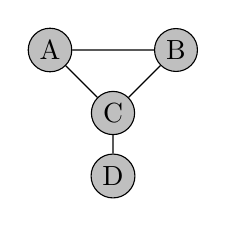
\begin{tikzpicture}[scale=0.8, every node/.style={circle, draw, fill=lightgray, inner sep=2pt}]
\node (A) at (0,2) {A};
\node (B) at (2,2) {B};
\node (C) at (1,1) {C};
\node (D) at (1,0) {D};
\draw (A)--(B);
\draw (A)--(C);
\draw (B)--(C);
\draw (C)--(D);
\end{tikzpicture}
\end{center}

The graph can be represented as an adjacency list:
\begin{verbatim}
graph = {
    "A": ["B", "C"], "B": ["A", "C"], "C": ["A", "B", "D"], "D": ["C"]
}
\end{verbatim}

Apply the \texttt{BronKerbosch} algorithm (without pivoting) to find all maximal cliques:

\begin{enumerate}
    \item Write the initial call to the algorithm (i.e., the starting values of $R$, $P$, and $X$).
    \item Trace the first two recursive calls that lead to reporting a maximal clique. Show the values of $(R, P, X)$ at each step.
    \item List all maximal cliques of $G$. Which one(s) are maximum?
\end{enumerate}


\end{problem}


\end{document}

